\section{Consenso Promedio en Sistemas Holonómicos}
\onecolumn
\subsection{Grafo completamente conexo}
Protocolo de consenso de vecino más cercano de Jadbabaie et al.~\cite{jadbabaie2003}, con agentes integradores en el plano:
\begin{align*}
    \dot{\mathbf{x}}_i &= \mathbf{u}_i \\[6pt]
    \mathbf{u}_i &=
    \underbrace{\sum_{j \in \mathcal{N}_i} a_{ij}\,(\mathbf{x}_j-\mathbf{x}_i)}_{\text{\footnotesize Atracción a los vecinos}}
\end{align*}

%Cuando los cuatro agentes se perciben entre sí, el grafo es conexo y el protocolo converge al promedio real de las posiciones iniciales, de acuerdo con las condiciones de convergencia de matrices estocásticas de Wolfowitz~\cite{wolfowitz1963}.


\section{Consenso Promedio en Sistemas Holonómicos}
\onecolumn
\subsection{Grafo completamente conexo}
El protocolo converge al promedio real de las posiciones iniciales, de acuerdo con las condiciones de convergencia de matrices estocásticas de Wolfowitz~\cite{wolfowitz1963}.

\begin{figure}[H]
    \centering
    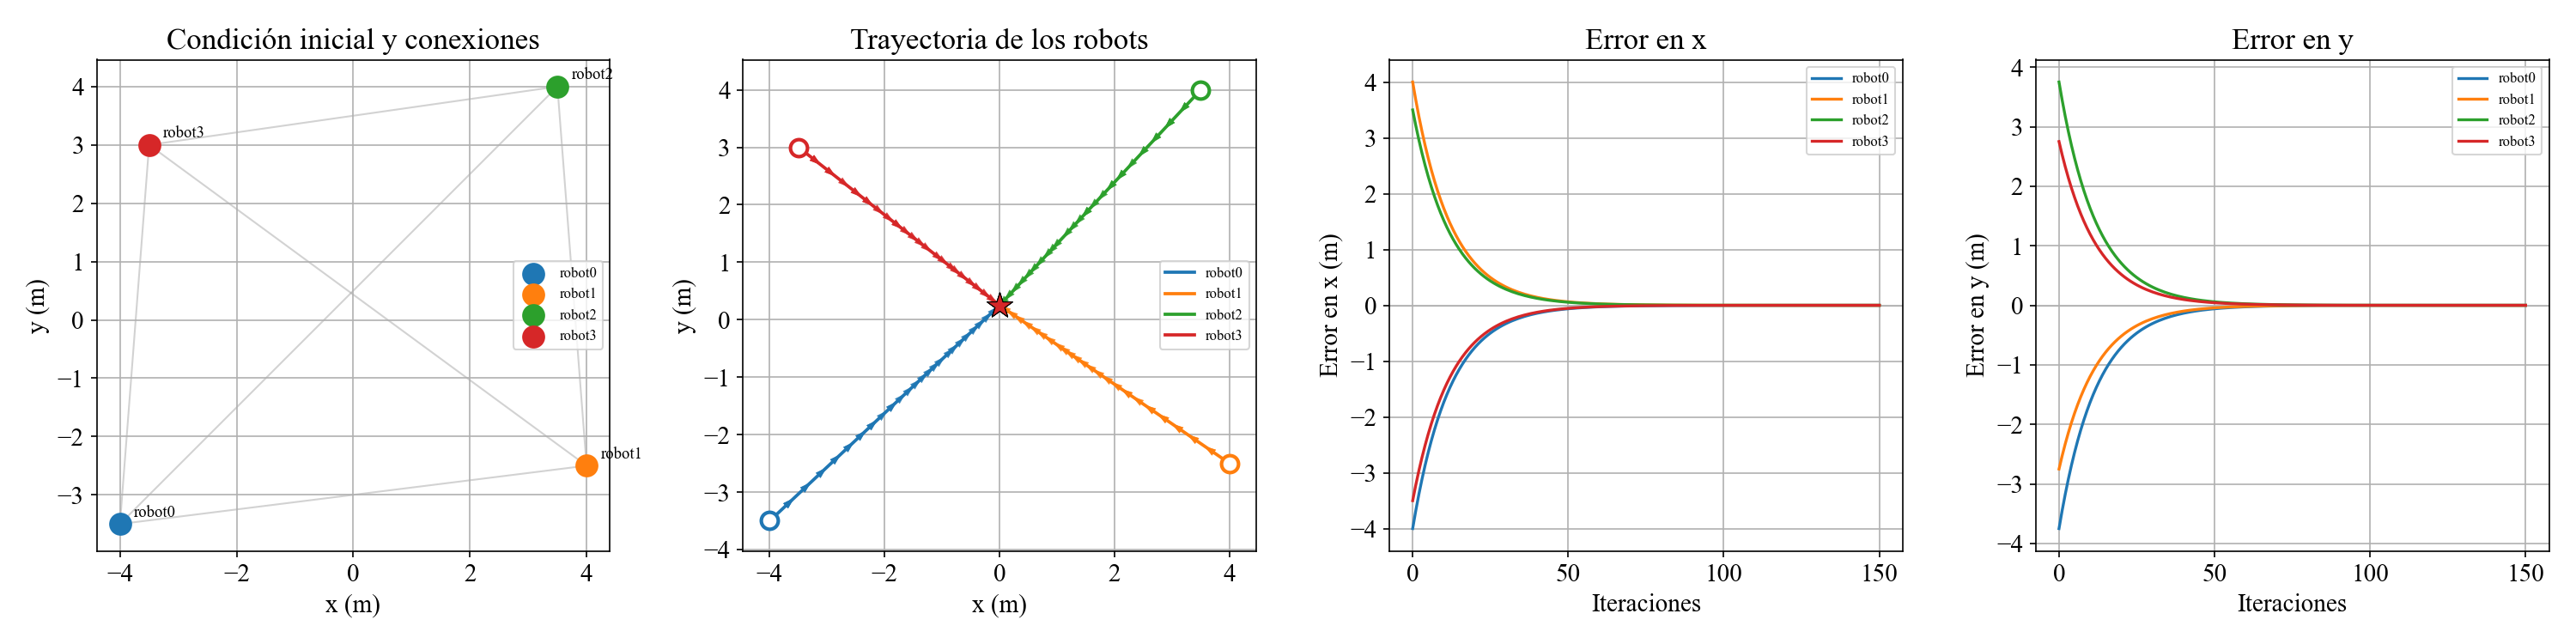
\includegraphics[width=\linewidth]{Pics/consenso_promedio_fully (1).png}
    \caption{Con grafo completamente conexo, los cuatro agentes convergen al promedio real de sus posiciones iniciales.}
    \label{fig:consenso_fully}
\end{figure}
